\documentclass[BTech]{iitmdiss}

\usepackage{lmodern}
\usepackage[scaled=0.8]{beramono}
\usepackage{t1enc}

\usepackage{graphicx}
\usepackage{epstopdf}
\usepackage[hypertex]{hyperref}
\usepackage{amsmath}
\usepackage{amssymb}
\usepackage{fancyvrb}
\usepackage[ruled,lined,commentsnumbered]{algorithm2e}
\usepackage{color}
\usepackage{listings}

\VerbatimFootnotes
\graphicspath{ {./images/} }

\captionsetup{font=footnotesize}

\definecolor{mygreen}{rgb}{0,0.6,0}
\definecolor{mygray}{rgb}{0.5,0.5,0.5}
\definecolor{mymauve}{rgb}{0.58,0,0.82}
\lstset{
	backgroundcolor=,                      % choose the background color; you must add \usepackage{color} or \usepackage{xcolor}
	basicstyle=\ttfamily,                  % the size of the fonts that are used for the code
	breakatwhitespace=false,               % sets if automatic breaks should only happen at whitespace
	breaklines=true,                       % sets automatic line breaking
	captionpos=b,                          % sets the caption-position to bottom
	commentstyle=\itshape\color{mygreen},  % comment style
	frame=L,                               % adds a frame around the code
	keepspaces=true,                       % keeps spaces in text, useful for keeping indentation of code (possibly needs columns=flexible)
	keywordstyle=\color{blue},             % keyword style
	language=C++,                          % the language of the code
	numbers=left,                          % where to put the line-numbers; possible values are (none, left, right)
	numbersep=10pt,                        % how far the line-numbers are from the code
	numberstyle=\tiny\color{mygray},       % the style that is used for the line-numbers
	rulecolor=\color{black},               % if not set, the frame-color may be changed on line-breaks within not-black text (e.g. comments (green here))
	showspaces=false,                      % show spaces everywhere adding particular underscores; it overrides 'showstringspaces'
	showstringspaces=false,                % underline spaces within strings only
	showtabs=false,                        % show tabs within strings adding particular underscores
	stepnumber=2,                          % the step between two line-numbers. If it's 1, each line will be numbered
	stringstyle=\color{mymauve},           % string literal style
	tabsize=4,                             % sets default tabsize to 2 spaces
	title=\lstname,                        % show the filename of files included with \lstinputlisting; also try caption instead of title
	xleftmargin=\parindent
}

% For the underbar vector notation, without losing the italics
\newcommand{\ue}[1]{\underbar{\emph{#1}}}

% For aligning subscripts and superscripts in correlation expressions
\newcommand{\corr}[2]{#1^{} #2^*}

% For inserting a blank page
\newcommand{\blankpage}[0]{
  \newpage
  \null
  \thispagestyle{empty}
  \newpage
}


\begin{document}

\title{A MODULARIZED OFDM STACK \\
       FOR COMMUNICATION USING \\
       UNIVERSAL SOFTWARE \\
       RADIO PERIPHERALS}

\author{PRAVEEN VENKATESH}

\date{JUNE 2014}
\department{ELECTRICAL ENGINEERING}

\maketitle

\blankpage
\certificate

\vspace*{0.5in}

\noindent This is to certify that the thesis titled {\bf A Modularized OFDM
Stack for Communication using Universal Software Defined Radio Peripherals},
submitted by {\bf Praveen Venkatesh}, to the Indian Institute of Technology,
Madras, in partial fulfillment of the requirements for the award of the degree
of {\bf Bachelor of Technology}, is a bona fide record of the work done by him
under our supervision. The contents of this thesis, in full or in parts, have
not been submitted to any other Institute or University for the award of any
degree or diploma.

\vspace*{1.5in}

\begin{singlespacing}
\hspace*{-0.25in}
\parbox{2.5in}{
	\noindent {\bf Prof.~Radhakrishna~Ganti} \\
	\noindent Research Guide \\
	\noindent Assistant Professor \\
	\noindent Dept. of Electrical Engineering\\
	\noindent IIT Madras - 600 036 \\
}
\hspace*{1.0in}
\end{singlespacing}

\vspace*{0.25in}

\noindent Place: Chennai \\
Date: 13 June, 2014


\blankpage
\acknowledgements

I'd sincerely like to thank my guide, Prof.\ Radhakrishna Ganti, for always
being there whenever I had a problem. I don't think I could have asked for
anything more in a guide, considering how he's physically sat alongside me,
reading obscure code and helping me figure out the problems.

Second, I'd like to thank Arjun for helping me through this entire journey. He,
too, has always been there when I needed someone to bounce ideas off, to check
my code, or otherwise help me figure out some problem.

I'd like to thank Prof.\ HSR for giving me some useful advice when I needed it,
and for being supportive when I chose to make the switch to Comm. I'd also like
to thank the other members of my lab, for making it a pleasant (if, at times,
somewhat PJ-filled) working environment.

Last, but not the least, I'd like to thank my family for giving me the freedom
to choose anyhow I wished, and for being fully supportive of any decision I
took.

\blankpage
\abstract

\noindent \textsc{keywords} \hspace*{0.5em} \parbox[t]{4.4in} {Orthogonal
Frequency Division Multiplexing; Timing Synchronization; Universal Software
Defined Radio Peripheral; Log Likelihood Ratio, Joint Trellis Shaping; Dirty
Paper Coding}

\vspace*{24pt}

\noindent This report outlines the theory behind, the working of, and the
design decisions that went into the creation of an OFDM stack and a few other
modules that were constructed primarily as component blocks of a larger
project aimed at implementing and demonstrating a real-time Dirty Paper Coding
framework in a base-station-with-two-users environment. The report aims to be
used as a reference design document for future generations of this framework.

\blankpage
\begin{singlespace}

\tableofcontents
\thispagestyle{empty}

\listoffigures
\addcontentsline{toc}{chapter}{LIST OF FIGURES}

\end{singlespace}

\blankpage
\abbreviations

\noindent
\begin{tabbing}
	xxxxxxxxxxx \= xxxxxxxxxxxxxxxxxxxxxxxxxxxxxxxxxxxxxxxxxxxxxxxx \kill
	\textsc{ofdm} \> Orthogonal Frequency Division Multiplexing \\
	\textsc{usrp} \> Universal Software Defined Radio Peripheral \\
\end{tabbing}

\blankpage

%%%%%%%%%%%%%%%%%%%%%%%%%%%%%%%%%%%%%%%%%%%%%%%%%%%%%%%%%%%%%%%%%%%%%%%%%%%%%%%

\clearpage

% The main text will follow from this point so set the page numbering
% to arabic from here on.
\pagenumbering{arabic}

%%%%%%%%%%%%%%%%%%%%%%%%%%%%%%%%%%%%%%%%%%%%%%%%%%%%%%%%%%%%%%%%%%%%%%%%%%%%%%%
% Chapters

\chapter{INTRODUCTION}
\label{chap:intro}

\section{Orthogonal Frequency Division \\ Multiplexing}

\subsection{Digital communication}
\label{subsec:digi-comm}

When transmitting digital data over a real (analog) channel, we typically first
convert the bit stream into a stream of complex symbols, using some kind of
modulation scheme. Following this, the symbols are pulse-shaped and upconverted
to the carrier frequency, real and imaginary parts of the symbols being encoded
in the in-phase and quadrature components of the carrier.

We can retrieve the complex symbols on the receiver side by performing matched
filtering followed by suitably sampling the analog data. In such a scenario,
the effects of the channel can also be viewed as purely digital operations on
the complex data stream. We can, therefore, work at the level of digital
abstraction, where we only deal with a discrete sequence of complex symbols.

\subsection{Channel effects}

The modulation scheme used will decide how robust the message will be against
channel effects. A simple but effective digital channel model has an impulse
response to model inter-symbol interference (caused due to multi-path effects
in wireless transmission, for example) and an addition of white gaussian noise.
Simple modulation schemes such as QAM do not fare well in such a channel,
however, due to ISI.

In order combat the effect of ISI in such cases, we would need to employ
computationally intensive decoding techniques such as the Viterbi algorithm.
Alternatives are to use sub-optimal equalization filters such as the
zero-forcing equalizer, but depending upon how many taps the channel has, these
filters could turn out to be extremely long, which once again, makes them
computationally intensive.

\subsection{OFDM solves the ISI problem}

OFDM is a modulation scheme that effectively solves the problem of ISI without
introducing heavy computational complexity. It does this by placing a block of
complex data symbols on adjacent narrow-band `subcarriers' in the frequency
domain. The transmitted data block is the inverse-FFT of the frequency domain
block. On the receiver side, each data block is converted back into frequency
domain by taking the FFT of the block.

Each block of data, after the inverse-FFT is performed, is prepended with a
cyclic prefix, which is a copy of the last few symbols. The length of this
cyclic prefix is equal to the number of taps in the channel's impulse response.
The cyclic prefix ensures that the effects of ISI remain limited to the same
data block and guards against pollution of symbols from adjacent data blocks.

With this framework, the ISI of the channel gets expressed in frequency domain
as frequency-selective fading, with each subcarrier seeing a different gain.
If we have a model of the channel in frequency domain, (by taking the FFT of
the channel taps), then we can reverse the effects of ISI completely by simply
dividing each received subcarrier symbol by the channel response at that
subcarrier.

%%%%%%%%%%%%%%%%%%%%%%%%%%%%%%%%%%%%%%%%%%%%%%%%%%%%%%%%%%%%%%%%%%%%%%%%%%%%%%%

\section{The USRP and the UHD API}

The USRP platform is a computer-hosted software-defined radio. In one sentence,
the USRP allows you to work at the level of digital abstraction alluded to in
subsection~\ref{subsec:digi-comm}. The device is connected to the computer
using either an ethernet cable or a USB 3.0 cable (depending upon the USRP
model used), and one can interface it to one's program by using the open source
UHD API.

Different USRP boards can work at different frequencies and have different
rates. The devices have the capability to act as a full transceiver. But at
least two distinct devices are required in order to perform experiments where
data is to be transmitted and received.

The UHD API can be used to interface with the USRP from a C++ program. The API
provides classes and methods to set up the USRP device with the desired
frequency, rate and gain settings. One can instantiate a transmit- or receive-
streamer to send or receive data in the form of a complex data stream.

In this project, the UHD API has been made use of extensively. The use of the
API has been restricted to two modules, namely the USRP Transmitter module and
the USRP Receiver module. These are described in
subsections~\ref{subsec:usrp-transmitter} and~\ref{subsec:usrp-receiver}.

\chapter{TIMING ANALYSIS}
\label{chap:timing}

%%%%%%%%%%%%%%%%%%%%%%%%%%%%%%%%%%%%%%%%%%%%%%%%%%%%%%%%%%%%%%%%%%%%%%%%%%%%%%%

\section{Packet detection}

Timing analysis is used to determine the point in time where the packet starts.
This is also a method to recognize \emph{whether} a packet has arrived or not.
In the current scheme, the packet detection module uses the Schmidl and Cox %(TODO: Put citation here)
method for timing analysis.

\subsection{The Schmidl and Cox algorithm}

For the receiver to be able to pick out a packet from ambient noise and
interference, the transmitted packet must be designed for detection. All
transmitted packets have a \emph{preamble}, which consists of two identical
halves. Each half is a pseudo-random-number sequence. The correlation of each
half with with other (independent and hence uncorrelated) signals is expected
to be low. However, its correlation with the other half will be high. Moreover,
this property is well-maintained even when the preamble is passed through an
ISI channel with additive white gaussian noise.

In other words, we can detect the start of a packet by correlating two adjacent
windows, each having half the size of the preamble, with each other. The point
where this correlation value becomes high can be taken to be the start of the
packet.

% TODO: Insert plot of preamble (real and imaginary) here
% TODO: Insert a picture of the two windows correlating received data

The metric used to determine whether or not the correlation value is high
enough is the normalized cross-correlation, defined as
$$ \text{Metric} = \frac{|\text{Cross-correlation of the two windows}|^2}
                        {\text{Product of the autocorrelations of the windows}}
$$

% TODO: Insert a picture of the metric over the data

\subsection{Running correlation on the receive buffer}

In order to efficiently perform a running correlation of adjacent windows over
an entire receive buffer, we minimize the number of computations performed. On
moving one step, we add the latest correlation point and subtract the oldest
correlation point.

Let $\ue{x}$ and $\ue{y}$ be complex vectors corresponding to the symbols in
the left half-window and the right-half-window respectively. Let $n$ be the
half-window size. After moving one time step, let these windows be denoted by
the complex vectors $u$ and $v$ respectively.  We thus have $u_i = x_{i+1}$ and
$v_i = y_{i+1}$ for $i = {1, 2, \ldots n-1}$.

Let $c_{old}$ be the correlation of $x$ with $y$, and $c_{new}$ be the
correlation of $u$ with $v$. That is,
$$ c_{old} = \corr{\ue{x}}{\ue{y}} = \sum_1^n{\corr{x_i}{y_i}} $$
$$ c_{new} = \corr{\ue{u}}{\ue{v}} = \sum_1^n{\corr{u_i}{v_i}} $$
where $^*$ denotes complex conjugation. We can then write $c_{new}$ in terms of
$c_{old}$ as follows:
\begin{align}
	c_{new} &= \sum_1^{n-1}{\corr{u_i}{v_i}} + \corr{u_n}{v_n} \\
	        &= \sum_2^n{\corr{x_i}{y_i}} + \corr{u_n}{v_n} \\
	        &= \sum_1^n{\corr{x_i}{y_i}} - \corr{x_1}{y_1} + \corr{u_n}{v_n} \\
	        &= c_{old} - \corr{x_1}{y_1} + \corr{u_n}{v_n}
\end{align}

This way, once we have acquired the correlation of the first $n$ symbols, the
correlation of subsequent windows is an $\mathcal{O}(1)$ process.

%%%%%%%%%%%%%%%%%%%%%%%%%%%%%%%%%%%%%%%%%%%%%%%%%%%%%%%%%%%%%%%%%%%%%%%%%%%%%%%

\section{The DC offset problem}

\subsection{Discovering the DC offset}
\subsection{Eliminating the DC offset}
\subsection{Running correlations with DC offset elimination}

%%%%%%%%%%%%%%%%%%%%%%%%%%%%%%%%%%%%%%%%%%%%%%%%%%%%%%%%%%%%%%%%%%%%%%%%%%%%%%%

\section{Practical considerations}

\subsection{Cross-correlation cut-off for noisy regions}
\label{sec:cross-corr-cut-off}

We expect the absolute value of the cross-correlation of the two windows to be
much lower than the product of their autocorrelations. However, we found that
the value of the metric tended at times to be quite large, and even comparable
to the threshold used to determine the presence of a packet.

A possible reason for this might be the accumulation of errors due to the
running correlation algorithm being employed. In the regions of noise, both the
autocorrelation and cross-correlation values are low, however, random
fluctuations in the noise and in the error could sometimes cause them to become
roughly of the same order of magnitude.

In order to prevent erroneous packet detection in noisy regions, we introduced
a cut-off based on the absolute value of the cross-correlation. This cut-off
value must be empirically determined. If the absolute value of the
cross-correlation is less that the cut-off, we manually set the running
cross-correlation at the point to be zero, and skip all other checks for the
packet.

%TODO: Put pseudocode / actual code snippet here

\subsection{Violation of Cauchy-Schwarz inequality}

We discovered that at certain instances, for example when searching for the
preamble towards the end of a previous frame, the value of the metric exceeded
unity. In a strict mathematical sense, this is impossible, since
cross-correlation is an inner product operation, and the Cauchy-Schwarz
inequlity guarantees that
$$ \langle \ue{u}, \ue{v} \rangle ^2 \leqslant |\ue{u}||\ue{v}| $$
Nevertheless, the situation was observed. On closer inspection, we found that
at the edge of the frame, the values of the complex symbols dropped rapidly. In
such a situation, it took time for the cross-correlation value to settle (time
for the accumulated errors to diminish in comparison to the cross-correlation
value itself), whereas the autocorrelation values settled faster. This caused
the cross-correlation value to exceed the autocorrelation product, thus giving
a metric value greater than unity.

When checking for the preamble itself, we gave allowances for errors causing
the metric value to exceed unity. But in the situation described above, this
occurred with far larger deviations than we might expect due purely to floating
point error. In fact, the error was the accumulated error in the algorithm
itself. In such situations also, we manually set the cross-correlation value to
zero to avoid further propagation of this error.

%TODO: Insert code snippet

\subsection{Fine metric}

When searching for the preamble in the body of a previous frame, we sometimes
found that the value of the metric exceeded the threshold. Essentially, the
values of the complex symbols within the frame depends on the data being
transmitted. It might so happen that the data produces a short repeating
pattern of the same length as the preamble in the bulk of the frame. In such a
sitation, the timing synchronizer will erroneously detect a packet in the
middle of a frame.

This is because, so far, we have only correlated the first half of the preamble
with the second half in the received vector. We never correlated the received
symbols with the actual preamble values themselves (which are fixed, and thus
known at the receiver). It may not be possible to simply increase the threshold
until this stops happening, since the threshold value is determined by the
amount of noise in the system. %TODO: Insert ref to appendix with tuning.

To fix this issue, the fine metric is computed by correlating the first window
with the first half of the expected preamble. This is only done when the coarse
metric exceeds the threshold, since it is an expensive operation and since we
cannot use a running correlation algorithm to compute it. The fine metric value
has its own threshold, which is used as a second-pass for ensuring the presence
of an authentic preamble.

Note that even in the presence of an ISI channel, the fine metric will pick up
the most dominant channel tap. If $\ue{p}$ is the preamble vector and $\ue{h}$
is the channel, then the received preamble is
$$\ue{y} = \ue{p} * \ue{h}$$
This received vector is now correlated with the preamble itself, so that the
fine metric peaks at $\text{argmax}(\ue{h})$ with a peak value of
$\text{max}(\ue{h})$.

%TODO: Insert fine metric plot

%%%%%%%%%%%%%%%%%%%%%%%%%%%%%%%%%%%%%%%%%%%%%%%%%%%%%%%%%%%%%%%%%%%%%%%%%%%%%%%

\section{Further optimizations}

\subsection{Stopping correlation after threshold breach}
\subsection{Discarding the found frame block}

% TODO: Appendix on tuning the timing synchronizer

\chapter{THE MODULARIZED OFDM STACK}
\label{chap:ofdm-stack}

%%%%%%%%%%%%%%%%%%%%%%%%%%%%%%%%%%%%%%%%%%%%%%%%%%%%%%%%%%%%%%%%%%%%%%%%%%%%%%%

\section{The goal}

Ideally, we wish to achieve a level of abstraction over the physical layer that
allows us to operate at the level of bit-streams. We would like to transmit the
bits with almost no knowledge of the underlying layer and mechanism. Suppose
bits were stored as arrays of \lstinline!char! elements, we would like to
transmit them with a single function call:

\begin{lstlisting}
	char *bits;
	// ... fill in the array
	transmit(bits);
\end{lstlisting}

Underlying this, there needs to be configurability. That is, if desired, we
should be able to break the abstraction and set options on the transmitter and
receiver. One way of doing this might be through a configuration file. But this
would mean that we cannot change parameters dynamically. So the underlying
framework should allow us to access internals in the code, if desired:

\begin{lstlisting}
	double freq = get_transmit_frequency();
	if(freq != 9e6) {        // Change freq to 900 MHz.
		change_transmit_frequency(9e6);
	}
\end{lstlisting}

In order to achieve this, we need to have a well-abstracted and modularized
code base. The data should be disconnected from the code to the maximum extent
possible. Different components of the code should be loosely coupled, that is,
there should be minimal interdependence between different modules, and they
should be maximally self-contained.

While, at present, the OFDM stack does not meet this ideal, one may at least
say that it has plotted itself a course and is well on its way.

%%%%%%%%%%%%%%%%%%%%%%%%%%%%%%%%%%%%%%%%%%%%%%%%%%%%%%%%%%%%%%%%%%%%%%%%%%%%%%%

\section{The modules}

The program has been functionally broken up into modules, as shown in
figure~\ref{fig:modules}.

%TODO: Figure showing modularity

A more detailed description of each of these modules follows.

\subsection{The mapper}

The mapper converts a sequence of bits into one of complex symbols. The reason
this has been kept outside of the OFDM framework is that different applications
have different requirements on the kinds of complex symbols generated.

Mapping may be performed on a coded bit stream, in which case it may be
sufficient to use a standard constellation to perform mapping. But in the
implementation of DPC, for example, we pre-subtract the expected interference
from another user. As a result, we do not transmit any fixed constellation
points. Any point in the available complex plane may be transmitted as a
symbol.

It is therefore best to allow for different kinds of mappers. In the interest
of keeping the OFDM framework loosely coupled with the mapping framework, the
two have been made into separate modules. The default mapper can now be
`unplugged' and a new, custom-defined mapper can be `plugged in' to the code.

\subsection{The OFDM Modulator}
\label{subsec:ofdm-modulator}

The OFDM Modulator converts a sequence of complex symbols into a sequence of
packets. Several configuration details come into play here, such as the number
of symbols that go into each frame, details of the preamble used in the frame,
etc.

In order to maintain a list of these values that can be used by the various
functions that fall under the ambit of the OFDM Modulator, the modulator has
been made into a class. The data members of the class allow for encapsulation
and abstraction, so that the settings are exposed for change only if desired.

A set of default parameters are automatically loaded when the object is
instantiated. Following this, settings can be changed by setting them manually
if desired. This can be done directly by assignment, since all data members are
public. After this, the object has to be initialized using the
\lstinline!initialize()! member function. This allocates memory and creates
\lstinline!fftw_plan!s. In a multi-threaded environment, this operation is not
thread-safe, and therefore must be completed before thread-creation.

In the transmit loop, the \lstinline!modulate()! call does the job of making
the symbols passed to it into packets. It returns a packet, which is a sequence
of time-domain complex symbols that can be transmitted using some sort of
transmitter.

\subsection{The USRP Transmitter}

The USRP Transmitter module is an encapsulated version of the UHD API for
transmission. As described in subsection~\ref{subsec:ofdm-modulator}, some
default parameters are loaded upon instantiation, which can be changed later.
Further, the \lstinline!add_options()! member function can be used to let the
module add its own set of options to the command line, via the
\lstinline!boost! \lstinline!program_options! module. All this must be
followed up with an \lstinline!initialize()! call.

The transmitter uses the \lstinline!transmit()! function to transmit symbols.
Usually, one packet of complex symbols (as received from the OFDM Modulator) is
transmitted at a time. However, there is really no such restriction. The
transmitter can be used independently of the OFDM modulator to transmit any
sequence of complex symbols.

\subsection{The USRP Receiver}

The USRP Receiver module is similar to the USRP Transmitter in all respects.
The \lstinline!receive()! call is used to receive a desired number of complex
symbols from the USRP.

\subsection{The OFDM Demodulator}

The OFDM Demodulator is the least independent of all the modules. It is also
the heaviest in terms of computational requirement and code size. The primary
reasons for the lack of its independence are the stringent requirements of the
timing analyser, given its working mechanism. It has a specific requirement on
the buffer size. Furthermore, in order to decrease the burden on the timing
analyser, we implemented frame-discarding, as described in
subsection~\ref{subsec:frame-discard}. This resulted in the use of the
unwieldy variables \lstinline!num_left_to_search! and
\lstinline!num_to_acquire!. These variables inevitably decrease the level of
independence of this module, because they force it to become coupled with the
process of acquisition of symbols (which is really different module's work), by
definition.

This module provides the \lstinline!demodulate()! member function to detect
whether or not packets are present in the given buffer, and if they are, then
to demodulate them and return a set of received complex symbols that should
have come from transmitted constellation points.

%%%%%%%%%%%%%%%%%%%%%%%%%%%%%%%%%%%%%%%%%%%%%%%%%%%%%%%%%%%%%%%%%%%%%%%%%%%%%%%

\section{Limitations}

While the modularized implementation has enabled plugging and unplugging of
various modules, there are still many things that this framework cannot do.

\subsection{Using two different kinds of frames}

It may sometimes be desirable to use two different kinds of frames, for eg.\ a
long data frame for transmitting information, and a short acknowledgement
frame, to tell the other side that a packet has been received. While the basic
structure is present for making use of two different kinds of frames, possibly
with different preambles or data masks, the implementation of the same is not
easy and requires some work on the part of the developer.

Currently, it is possible to create two or more different OfdmModulator and
OfdmDemodulator object pairs, and then manually specifying a different preamble
or data mask for each pair. Since all data members are public, they can be
directly changed after instantiation. An \lstinline!initialize()! call will
then allocate requisite memory, create \lstinline!fftw_plan!s and so on.

Modulation too, should not be a hassle. However, when calling the demodulate
function, there is some amount of coupling between the calling program and the
demodulator in the form of \lstinline!num_left_to_search! and
\lstinline!num_to_acquire!. If the \lstinline!frame_size!s of the two types
of frames are different, then during packet detection, we may get different
values of \lstinline!num_left_to_search! and \lstinline!num_to_acquire!
from each demodulator object. We would then have to create a temporary buffer
to manage the different requirements of \lstinline!num_left_to_search! and
\lstinline!num_to_acquire! for the two demodulators.

\subsection{Using single precision}

It is currently not possible to use single precision instead of double
precision, because the FFTW module in its present configuration uses only
double precision. While this by itself would not prevent us from using single
precision elsewhere, issues arise because at present, there are
\lstinline!reinterpret_cast!s between our flexible \lstinline!Complex! and
FFTW's less flexible \lstinline!fftw_complex! data types.

In order to use single precision everywhere, there is a need to refactor the
usage of FFTW, using preprocessor tricks to switch between
\lstinline!fftw_complex!, the double precision implementation and
\lstinline!fftwf_complex!, the single precision implementation, depending on
the value of a preprocessor variable.

\chapter{MODULES FOR DIRTY PAPER CODING}
\label{chap:dpc-modules}

%%%%%%%%%%%%%%%%%%%%%%%%%%%%%%%%%%%%%%%%%%%%%%%%%%%%%%%%%%%%%%%%%%%%%%%%%%%%%%%

\section{Log Likelihood Ratio computation}

There is a requirement for the computation of log-likelihood ratios prior to
decoding the constellation symbols. Furthermore, this log-likelihood ratio is
to be computed on a repeated constellation.

The reason for this is that while transmitting symbols (from a base station to
a user in a 2-user system) in the DPC framework, interference from user 2 has
to be pre-subtracted from the constellation symbol being transmitted for user
1. During this process, it is possible that the symbol that is finally to be
transmitted lies outside of the constellation boundary. In such a situation,
the symbol in question is removed and reintroduced on the other side of the
constellation. The operation can be likened to a modulo operation, pulling
symbols outside of an interval back into the interval by repeatedly subtracting
the interval size.

On the receiver side, for the computation of LLRs, it is essential for
correctness to consider the possibility that a symbol might actually have come
from an out-of constellation point, or effectively from the other side of the
constellation. For the purpose of LLR computation, therefore, we can assume
that the symbol came from a repeated grid of the constellation.

This has currently been implemented only for a repeated 256-QAM constellation.

\subsection{Approximation of LLR}

The likelihood ratio is defined for each received bit as the ratio of the
probability of the corresponding transmitted bit being a 1 to to that of it
being a 0. This probability is computed for a given known noise variance, which
must be estimated beforehand.

In a 256-QAM constellation, the received constellation symbol could have come
from any of the 256 constellation points. Each constellation point encodes 8
bits. So from one received 256-QAM constellation point, we get 8 LLR values. At
any given bit position, half the constellation points will correspond to 0 and
the other half to 1. For computing the exact LLR value, we consider the
probability of the bit having come from each of these constellation symbols.

Let $s_i$ be the transmitted constellation points and $r$ be the received
complex vector. We wish to compute the LLR for a given bit (position) $b$. Let
$S^0$ be the set of indices $i$ for which $s_i$ has a 0 at bit position $b$,
and $S^1$ be the set of indices for which $s_i$ has a 1 at bit position $b$.
Then, the LLR for bit $b$ of the received vector $r$ is
\begin{equation}
	\text{LLR}(b) = \text{log} \left (
		\frac{ \sum_{i \in S^0}{e^{- |s_i - r|^2 / (2 \sigma^2)}} }
		     { \sum_{i \in S^1}{e^{- |s_i - r|^2 / (2 \sigma^2)}} }
		\right )
\end{equation}
where $\sigma^2$ is the noise variance.

To compute the LLR for each bit thus becomes very expensive, because it
involves 256 exponentiation operations. Since these LLR values are used only as
guides in the LDPC decoder, we do not need the exact LLR values. It is
sufficient to have good approximations of the same.

To this end, we neglect all terms except the dominant one in the numerator and
denominator of the likelihood ratio expression. That is to say, we redefine the
likelihood ratio as the ratio of the probability that the given received bit is
a 1, given that it came from the nearest constellation point having a 1 at the
corresponding bit location, to the probability that the given received bit is a
0, given that it came from the nearest constellation point having a 0 at the
corresponding bit location.
\begin{align}
	\text{LLR}_{\text{approx}}(b) &= \text{log} \left (
		\frac{ e^{- |s_{i^*_0} - r|^2 / (2 \sigma^2)} }
		     { e^{- |s_{i^*_1} - r|^2 / (2 \sigma^2)} }
		\right ) \\
		&= \frac{|s_{i^*_1} - r|^2 - |s_{i^*_0} - r|^2}{2 \sigma^2}
\end{align}
where $i^*_0$ corresponds to the nearest constellation point with index in
$S^0$ and $i^*_1$ corresponds to the nearest constellation point with index in
$S^1$.

\subsection{Computation of the approximate LLR}

In order to compute the approximate LLR for a bit, we need only the distance to
the constellation points corresponding to the nearest 0 and the nearest 1 for
that bit. To simplify our approach, we rely on the fact that \emph{the
constellation points corresponding to the nearest 0 and the nearest 1 are the
same (constant) for all points (all possible receive vectors) within the
decision region of each transmitted constellation point}.

In other words, we can precompute the constellation points corresponding to the
nearest 0 and the nearest 1 for each transmitted constellation point and store
these values in a table.  Then, we only need to find out the nearest
constellation point corresponding to a receive vector. This will tell us the
nearest 0 and the nearest 1 corresponding to a receive vector. Subtracting the
squares of the distances gives us the required LLR value.

\subsection{Nearest constellation point in a repeated constellation}

In order to compute the approximate LLR, we need to find the nearest
constellation point to the received vector. This is equivalent to the operation
of slicing, or locating which decision region the given receive vector lies
within. The only difference is that we need to do this in a repeated
constellation setting. This, in fact, makes our job a whole lot easier, because
it enables us to use floor and modulo operations.

\begin{figure}[h]
	\centering
	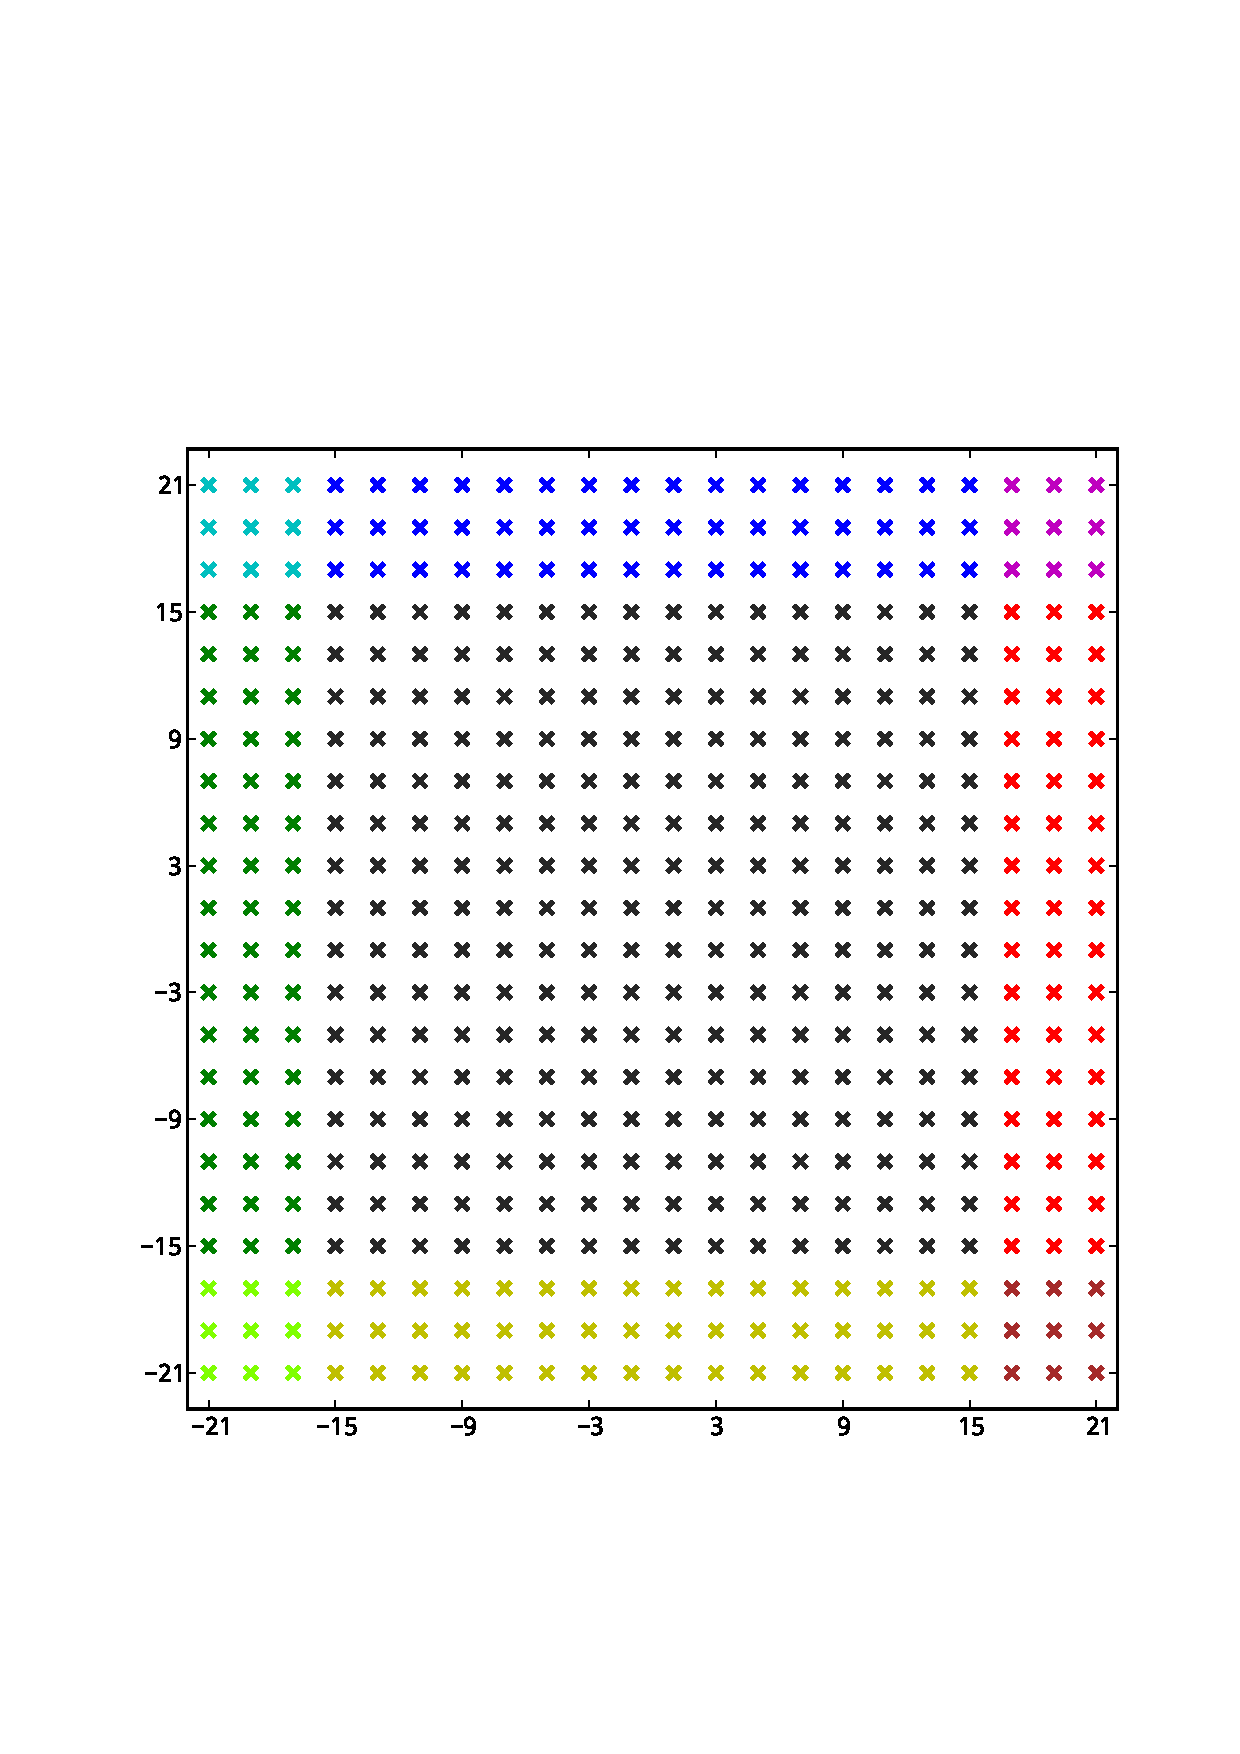
\includegraphics[width=0.8\textwidth]{256-qam-reptd-constln}
	\caption{Repeated 256-QAM constellation, prior to normalization. The
	         primary constellation is black, while its repetitions are coloured
	         variously.}
	\label{fig:256-qam-reptd}
\end{figure}

Consider the canonical 256-QAM constellation where constellation points are
located at odd points on the grid, from $-15$ to $+15$, on both real and
imaginary axes. On top of this, we have repetitions, so that the same
constellation is also present from $-47-15j$ to $-17+15j$ (left-bottom and
right-top corners of the constellation rectangle being used to denote
boundaries) on the left, from $-15+17j$ to $15+47j$ on the top, and so on in
all other directions (refer figure~\ref{fig:256-qam-reptd}).

Note that constellation points on $x=-17$ encode the same 8 bits as
constellation points on $x=+15$, and so on. This is the idea behind the
\emph{`modulo'} or the \emph{`repetition'}. This enables us to do the following
for slicing: we scale and translate the decision boundaries of the
constellation to the points of discontinuity of the floor function, and use the
floor function to achieve slicing. Following this, we use a modulo operation to
bring all repeated constellation points back into the primary constellation.

\begin{lstlisting}
	double x = creal(received_symbol);
	double y = cimag(received_symbol);
	// Move the received point back into the primary constellation
	x -= 32 * floor((x+16) / 32);
	y -= 32 * floor((y+16) / 32);
	// Find the index of the nearest constellation point
	int x_index = (int)(floor(x / 2) + 8);
	int y_index = (int)(floor(y / 2) + 8);
\end{lstlisting}

%%%%%%%%%%%%%%%%%%%%%%%%%%%%%%%%%%%%%%%%%%%%%%%%%%%%%%%%%%%%%%%%%%%%%%%%%%%%%%%

\section{Viterbi algorithm for Joint Trellis Shaping}

Joint Trellis shaping is aimed at minimizing the transmitted constellation
energy over a large number of constellation symbols. In order to do this with
greater ease, we use an almost-gray mapping scheme for the constellation.

The mapping for 256-QAM is based off the mapping for 16-PAM. The first four
bits are mapped using a 16-PAM constellation to get the real part of the
256-QAM constellation point. Similarly, the next four bits are used to get the
imaginary part.

%TODO: Insert 16-PAM constellation.

The 16-PAM constellation used is almost-Gray coded. Notice that the last three
bits read the same when sarting at $-15$ and going right, and when starting at
$+1$ and going right. The first bit, i.e.\ the sign bit, can therefore be used
to position the constellation point towards the centre of the constellation
(with lower energy) or towards the edge of the constellation (with higher
energy).

The point of trellis shaping is to choose sign bits in such a way as to
minimize the overall constellation energy, averaged over many transmitted
symbols. In the case of DPC, we need to perform joint trellis shaping, wherein
we minimize the overall average constellation energy of two users. To achieve
this the optimal way, we make use of the Viterbi algorithm.

\subsection{Shaping using the trellis}

The Viterbi algorithm is used to find the optimal sequence of signed bits to
minimize the overall energy of the transmitted symbols. Different choices of
signed bits make different paths in the trellis. The branch metric corresponds
to the energy of the constellation point generated by a certain choice of sign
bits. Thus, by finding the optimal path, we minimize the overall transmit
energy.

\subsection{Implementing the Viterbi algorithm}

In the Viterbi algorithm, edge weights (or the branch metrics) denote the
`cost' of choosing a certain path and node weights denote the accumulated
minimum cost of reaching that particular node.

We start by assigning a node weight of zero to the left-most states in the
trellis. Following this, at `time step', we need to compute the edge weights.
Given a set of input bits, we need to evaluate all possible choices of sign
bits. Each edge's weight is then the transmitted energy of the corresponding
constellation point that results from choosing that particular sign bit.Next,
we need to update the node weights of the next time step. This is done by
choosing, for each node, an input edge, which yields the least cost after
adding its branch metric with the corresponding source node's weight. A summary
of this algorithm in pseudocode is presented in algorithm~\ref{alg:viterbi}.

\begin{algorithm}[h]
	\SetKwData{Edge}{edge} \SetKwData{ToNode}{to\_node} \SetKwData{FromNode}{from\_node} \SetKwData{StateDiagram}{state\_diagram} \SetKwData{Weight}{weight}
	\SetKwData{MinNode}{min\_node} \SetKwData{PrevNode}{prev\_node} \SetKwData{Path}{path} \SetKwData{Node}{node}
	\SetKwFunction{Min}{Min} \SetKwFunction{Compute}{Compute}
	\SetKwInOut{Input}{input} \SetKwInOut{Output}{output}

	\Input{\StateDiagram;$\;$\emph{input bits for \Edge.\Weight computation}}
	\Output{\Path}
	\BlankLine
	\emph{initialize start node weights to $0$}\;
	\emph{initialize all other node weights to $\infty$}\;
	\ForAll{time steps} {
		\ForEach{\Edge in \StateDiagram} {
			\Compute{\Edge.\Weight}\;
			\If{\Edge.\ToNode.\Weight $>$ \Edge.\FromNode.\Weight $+$ \Edge.\Weight} {
				\Edge.\ToNode.\Weight $\leftarrow$ \Edge.\FromNode.\Weight $+$ \Edge.\Weight\;
				\Edge.\ToNode.\PrevNode $\leftarrow$ \Edge.\FromNode\;
			}
		}
	}
	\MinNode $\leftarrow$ \Min{final nodes}\;
	\Node $\leftarrow$ \MinNode\;
	\While{\Node not in start nodes} {
		\Path $\leftarrow$ \Node\;
		\Node $\leftarrow$ \Node.\PrevNode\;
	}
	\Return \Path\;
	\caption{The Viterbi algorithm}
	\label{alg:viterbi}
\end{algorithm}


%%%%%%%%%%%%%%%%%%%%%%%%%%%%%%%%%%%%%%%%%%%%%%%%%%%%%%%%%%%%%%%%%%%%%%%%%%%%%%%
% Appendices

\appendix

\chapter{TUNING THE TIMING SYNCHRONIZER}
\label{app:tuning}

\section{The requirement of tuning}

The timing synchronizer is makes several assumptions about the system in
question, and these assumptions are coded in the form of numerical parameters.
The values of these parameters must be determined empirically, by performing a
few measurements on the system. The `system', here, refers to the
transmitter-channel-receiver setup.

One possible use case scenario for tuning may be as follows: the synchronizer
is currently tuned for some frequency, but we desire to change the frequency of
operation by a large value. As a result, the expected degree of noise in the
system may increase. This could, potentially, cause erroneous packet detection
in a noisy patch, or more likely, cause a good packet to get dropped.

It is good to always keep a check on how many packets are being received, and
whether the rate at which they are being detected is equal to the rate at which
they are being transmitted. If it is found that the rate of reception of
packets is significantly lower, it is likely that the synchronizer needs to be
tuned.

%%%%%%%%%%%%%%%%%%%%%%%%%%%%%%%%%%%%%%%%%%%%%%%%%%%%%%%%%%%%%%%%%%%%%%%%%%%%%%%

\section{The debug files}

To run the program with debugging enabled for the timing synchronizer, clean
and re-compile the program with the make option \verb!DEBUG_TIMING_SYNC=true!
set, like so:
\lstset{language=}
\begin{lstlisting}
	$ make clean
	$ make cleandata
	$ make DEBUG_TIMING_SYNC=true
\end{lstlisting}
\lstset{language=C++}

Then, run the transmitter and receiver as usual, with the desired parameters,
for a short period of time. At the receiver end, the timing synchronizer should
output a bunch of \texttt{.out} files. Each of these is a binary file of
128-bit complex numbers, composed of two \lstinline!double!s. A list of these
files and descriptions of their content follows.

\begin{description}
	\item[\texttt{input\_data.out}] \hfill \\
		This file contains the received data stream as seen by the timing
		synchronizer. Only parts of frames, which are discarded once found (as
		described in subsection~\ref{subsec:frame-discard}), may be visible.
		Specifically, only the first half of the two-frame block is saved into
		this file. If a frame was found in the first half, then the parts of it
		that go into the second half are never `seen' by the timing
		synchronizer once the frame is discarded. \\
		All other debug files also share this particular property. Therefore,
		all debug files are of the same length, and their data can be overlaid
		on a plot (such as in figure~\ref{fig:metric}).
	\item[\texttt{abs.out}] \hfill \\
		This file contains the absolute value of the cross-correlation and the
		product of the autocorrelations of the correlation windows. The
		absolute value of the cross-correlation is stored in the real part of
		the data and the product of the autocorrelations is stored in the
		imaginary part of the data. For data location $i$, the two correlation
		windows start \emph{at} $i$ and extend $2n-1$ locations to its right.
	\item[\texttt{found\_packets.out}] \hfill \\
		This file contains the points where packets were found. If a packet
		was found at a given location, then this file contains a 1 at that
		position. At all other locations, it contains 0. \\
		While using 128-bit complex numbers may seem like a waste of space, it
		is convenient since it enables one to use the same mechanism to read
		all the debug files, as opposed to having to remember what number
		format needs to be used in each case.
	\item[\texttt{left\_avg\_new.out}] \hfill \\
		This contains the average, $\bar{x}$ of the left correlation window, as
		computed using the running average algorithm.
	\item[\texttt{right\_avg\_new.out}] \hfill \\
		This contains the average, $\bar{y}$ of the right correlation window,
		as computed using the running average algorithm.
	\item[\texttt{fine\_metric.out}] \hfill \\
		This contains the value of the fine metric (refer
		subsection~\ref{subsec:fine-metric}), wherever it had to be computed.
		At other locations, it contains 0.
\end{description}

%%%%%%%%%%%%%%%%%%%%%%%%%%%%%%%%%%%%%%%%%%%%%%%%%%%%%%%%%%%%%%%%%%%%%%%%%%%%%%%

\section{Performing tuning}

Check whether tuning is required by overlaying the input data, the metric and
the positions of found packets on a plot. In python, with the packages numpy
and matplotlib installed, this can be achieved as follows:

\lstset{language=Python}
\begin{lstlisting}
	import numpy as np
	import matplotlib.pyplot as plt

	a = np.fromfile('input_data.out', dtype=np.complex128)
	b = np.fromfile('abs.out', dtype=np.complex128)
	f = np.fromfile('found_packets.out', dtype=np.complex128)
	m = b.real / b.imag
	m = np.where(np.isfinite(m), m, np.zeros(m.size))
	
	plt.plot(abs(a), 'k')
	plt.plot(m)
	plt.plot(f.real)
	plt.show()
\end{lstlisting}
\lstset{language=C++}

\begin{figure}[h]
	\centering
	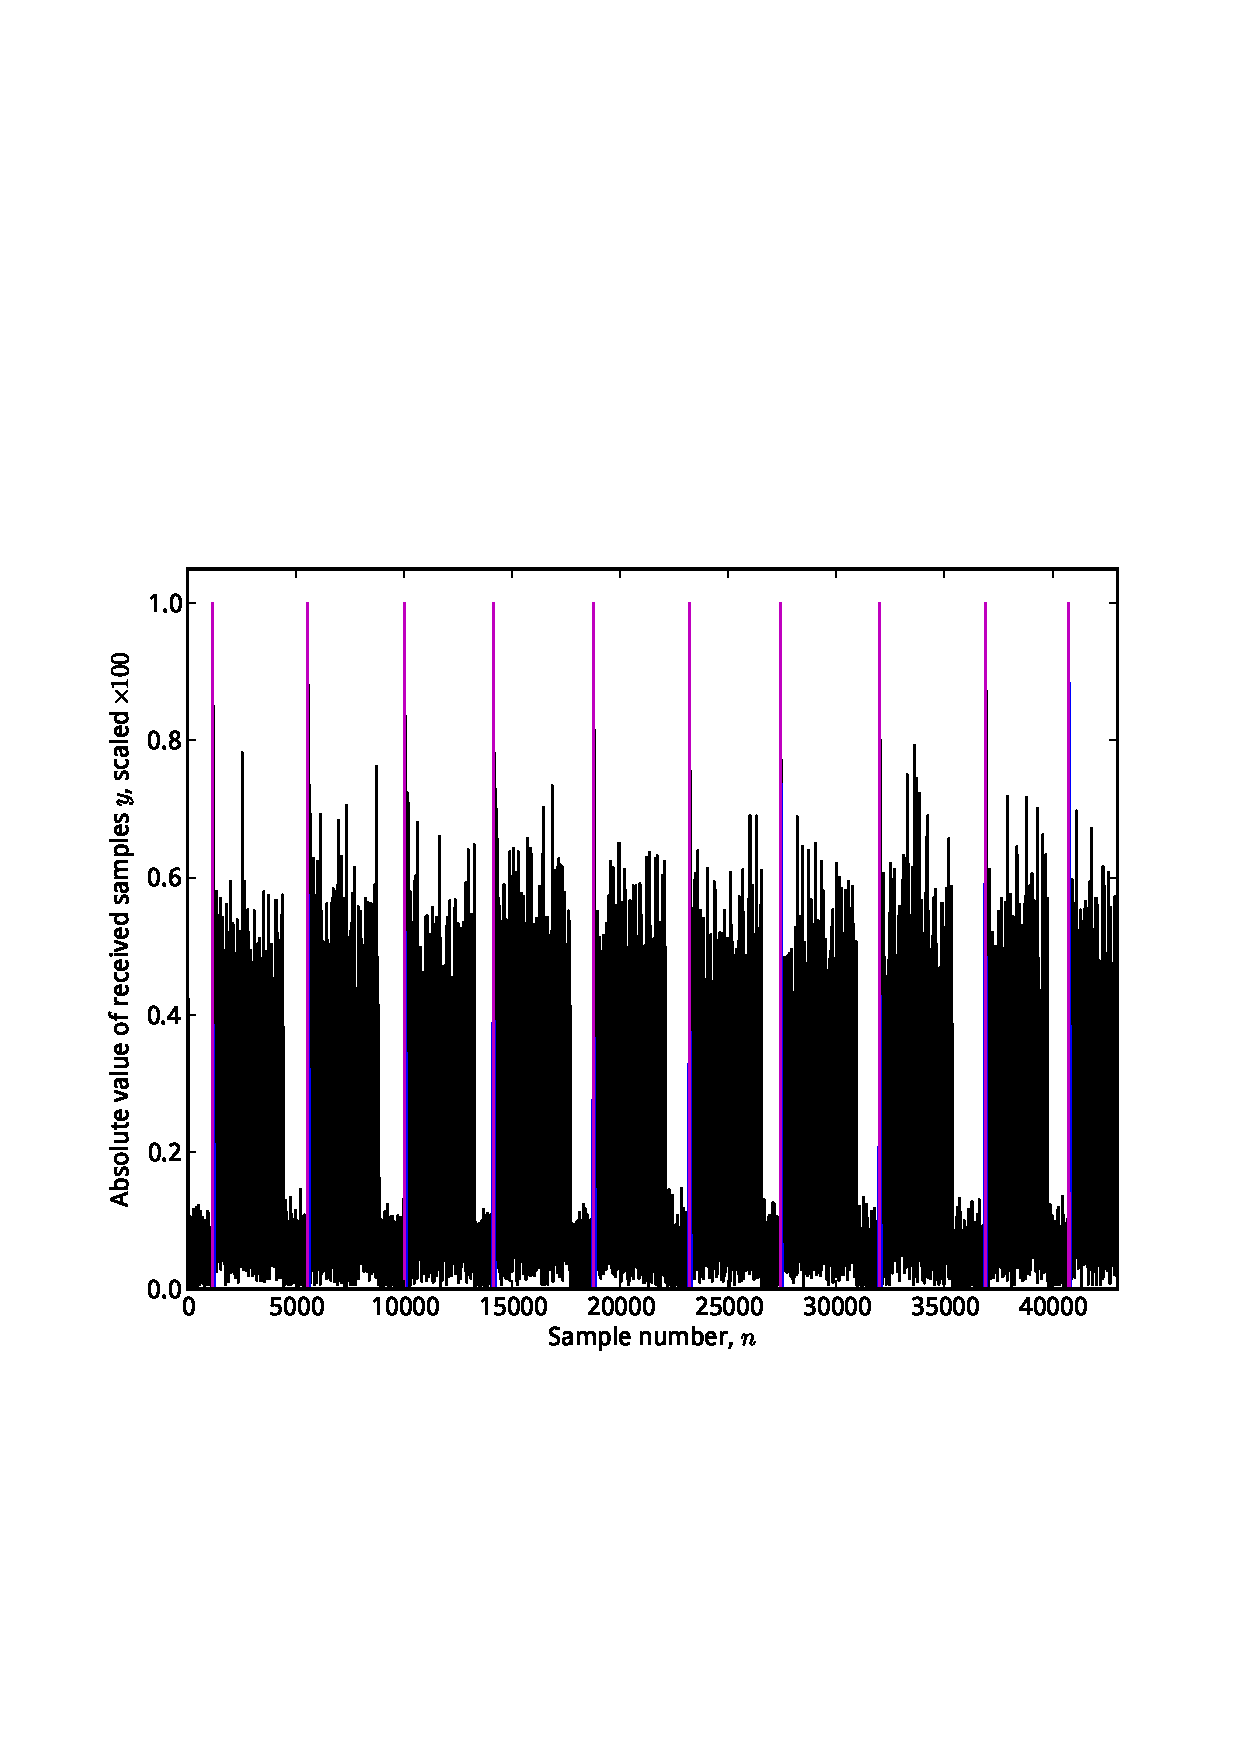
\includegraphics[width=0.8\textwidth]{packets}
	\caption{Packet stream after passing through the timing synchronizer}
	\label{fig:packets}
\end{figure}

This should, after suitable scaling, give a plot such as the one in
figure~\ref{fig:packets}. Note that all packets have been detected, as
indicated by the presence of the magenta line.

If there are several places where the packet fails to be detected, however,
then it calls for checking whether or not the metric exceeds the threshold. If
not, then the \lstinline!PACKET_THRESHOLD! parameter in the
\texttt{parameters.h} file needs to be changed so that the threshold is crossed
by the metric at the starting point of every packet, but is \emph{not} crossed
in other random locations.

Similarly, there may also be a need to modify the \lstinline!FINE_THRESHOLD!
parameter in the same file.

Furthermore, if the noise variance of the channel is high, it is possible for
the absolute value of the cross-correlation of noise to go above the
\lstinline!CROSS_CORR_THRESHOLD!. This may result in undesired effects, as
described in subsection~\ref{subsec:cross-corr-threshold}. Such a case can be
identified because the metric will be visible even in regions where there is no
packet.

In this case, plot the absolute value of the cross-correlation (the real part
of the data from the \texttt{abs.out} file) and overlay it on the data stream.
It should now be possible to set the \lstinline!CROSS_CORR_THRESHOLD! at a
value such that it is higher than the absolute value of the cross-correlation
of noise, but lower than the absolute value of cross-correlation of parts of a
packet.


%%%%%%%%%%%%%%%%%%%%%%%%%%%%%%%%%%%%%%%%%%%%%%%%%%%%%%%%%%%%%%%%%%%%%%%%%%%%%%%
% Bibliography

\begin{singlespace}
  \bibliography{refs}
\end{singlespace}

\end{document}
